\documentclass[12pt]{article}
\linespread{2}
\usepackage{times}
\usepackage{pgfplots}
\pgfplotsset{compat = newest}
\usetikzlibrary{positioning, arrows.meta}
\usepgfplotslibrary{fillbetween}
\usepackage{amsmath}
           \begin{document} 
                  \begin{center}
                     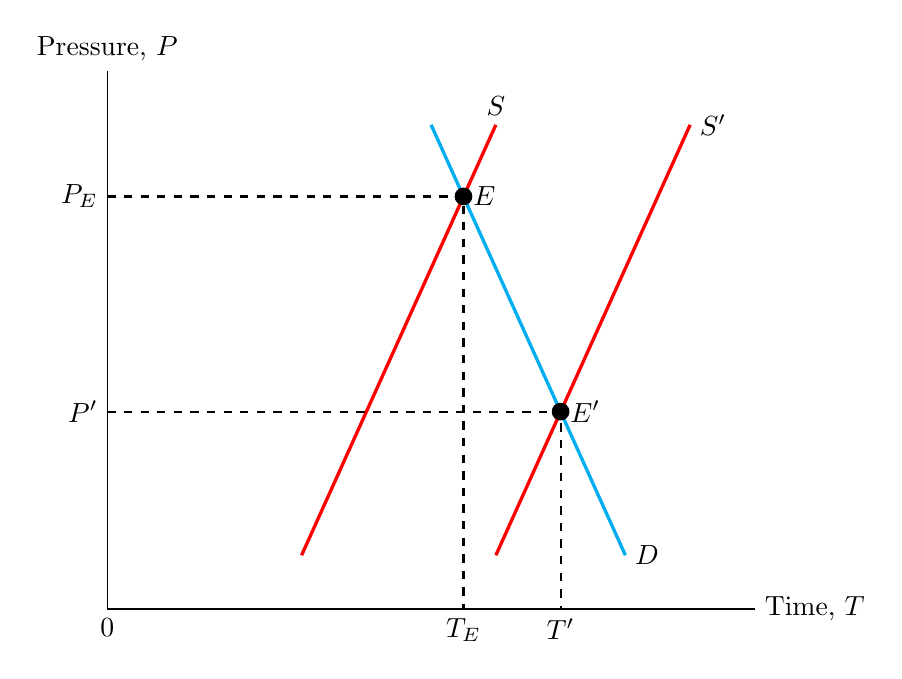
\begin{tikzpicture}
                          \begin{axis}[
                                       scale = 1.2,
                                       xmin = 0, xmax = 10,
                                       ymin = 0, ymax = 10,
                                       axis lines* = left,
                                       xtick = {0}, ytick = \empty,
                                       clip = false,
]

% Supply and demand curves
                         \addplot[color = cyan, very thick] coordinates {(5,9) (8,1)};
                         \addplot[color = red, very thick] coordinates {(3,1) (6,9)};
                         \addplot[color = red, very thick] coordinates {(6,1) (9,9)};


% Dashed lines
                         \addplot[color = black, dashed, thick] coordinates {(0, 7.67)
                                  (5.5, 7.67) (5.5, 0)};
                         \addplot[color = black, dashed, thick] coordinates {(0, 3.67) (7,
                                   3.67) (7, 0)};


% Coordinate points
                         \addplot[color = black, mark = *, only marks, mark size = 3pt]
                                  coordinates {(5.5, 7.67) (7, 3.67)};


% Labels
                         \node [right] at (current axis.right of origin){Time, $T$};
                         \node [above] at (current axis.above origin) {Pressure, $P$};
                         \node [right] at (5.5, 7.67) {$E$};
                         \node [right] at (7, 3.67) {$E^\prime$};
                         \node [right] at (8, 1) {$D$};
                         \node [above] at (6, 9) {$S$};
                         \node [right] at (9, 9) {$S^\prime$};
                         \node [left] at (0, 7.67) {$P_E$};
                         \node [left] at (0, 3.67) {$P^\prime$};
                         \node [below] at (5.5, 0) {$T_E$};
                         \node [below] at (7, 0) {$T^\prime$};
                         
                     \end{axis}
              \end{tikzpicture}
         \end{center}

               \textbf{Figure 12 }
  \end{document} 